% !TeX program = xelatex
% !TeX encoding = UTF-8
% Separate language revision R20261107-10; original source and PDF retained.
% Method first draft R20261106-06; Results R20261106-05; section plan R20261106-03.
% Standard natbib/BibTeX is used because local Biber cannot start; bibliography data remain in references.bib.
\documentclass[a4paper,11pt]{article}
\usepackage[english]{babel}
\usepackage{csquotes}
\usepackage{fontspec}
\usepackage[margin=2.5cm]{geometry}
\usepackage{amsmath,amssymb,graphicx,booktabs}
\usepackage{placeins}
\usepackage{indentfirst,tabularx}
\usepackage[font=small,labelfont=bf,justification=raggedright,singlelinecheck=false]{caption}
% A shared title/note hierarchy for every numbered figure and table.
\newcommand{\papercaption}[2]{\caption{\textbf{#1}\protect\newline\textit{Note.} #2}}
\usepackage{xurl}
\usepackage[hidelinks]{hyperref}
\usepackage[numbers,sort&compress]{natbib}
\graphicspath{{../figures/}}
% Consistent paragraph indentation, including the first paragraph after headings.
\setlength{\parindent}{1.5em}
\setlength{\parskip}{0pt}
\setlength{\emergencystretch}{1.5em}
\raggedbottom
\clubpenalty=10000
\widowpenalty=10000
\displaywidowpenalty=10000
\brokenpenalty=10000
% Keep text/equation paragraphs intact so floats cannot interrupt them.
\interlinepenalty=10000
\predisplaypenalty=10000
\postdisplaypenalty=10000
% Allow figures to share pages with their discussion rather than accumulating.
\setcounter{topnumber}{3}
\setcounter{totalnumber}{5}
\renewcommand{\topfraction}{0.9}
\renewcommand{\bottomfraction}{0.85}
\renewcommand{\textfraction}{0.08}
\renewcommand{\floatpagefraction}{0.75}
\setlength{\textfloatsep}{12pt plus 2pt minus 2pt}
\setlength{\floatsep}{10pt plus 2pt minus 2pt}
\makeatletter
\setlength{\@fptop}{0pt}
\setlength{\@fpsep}{12pt plus 2pt minus 2pt}
\setlength{\@fpbot}{0pt plus 1fil}
\makeatother
\title{Home-Win Prediction in International Football:\\
Team Strength, Historical Information, and Regional Variation}
\author{Names, student IDs, and classes to be confirmed}
\date{}
\begin{document}
\maketitle
\begin{abstract}
Historical home-win rates in international football may reflect team strength, match composition, and venue-related conditions. This study assesses their contribution to pre-match prediction. Comparisons across eras, match types, and regions use 24,917 non-neutral matches from 1980--2024. A dynamic model estimates strength from earlier results, including eligible neutral matches; a joint model combines the resulting strength distribution with match context. Retrospective chronological evaluation compares background-only, strength-only, and joint predictions on 21,413 matches from 1990--2024. The joint model reduced log loss by 16.12\% relative to background alone and 0.42\% relative to strength alone, achieving 70.01\% binary accuracy for home win versus non-home win. Historical-window comparisons identified a trade-off between fitting cost and probability quality, without establishing a universally optimal window. Regional diagnostics revealed differences in robustness and probability bias, distinct from descriptive geographic differences in home-win rates. A prospective release contains 52 fixtures, with 49 main predictions and three withheld under the venue rule; outcomes remain unevaluated. In the aggregate loss comparison, strength provided the larger improvement. Context contributed a smaller increment, whose interpretation remains conditional on model assumptions and the reuse of historical data during development.
\end{abstract}
\noindent\textbf{Keywords:} international football; pre-match strength; home-win probability; probabilistic prediction
% One compact front page, not a mostly empty title-only cover.
\clearpage
% !TeX root = ../main.tex
% Language revision R20261107-10; original retained in paper/sections/.
\section{Introduction}
\subsection{Motivation: From Historical Rates to Pre-Match Prediction}

Historical home-win rates in international football are sensitive to the teams, opponents, competitions, and periods included in a sample. A high rate may reflect a strong home team or a relatively weak set of opponents. Comparisons across regions or decades must therefore distinguish differences in match composition from differences in performance. For pre-match prediction, the relevant question is whether these historical patterns provide information beyond the teams' previous results.

Descriptive comparisons identify differences in observed home-win rates; predictive analysis assesses their value for subsequent matches. An aggregate difference may provide little additional information once team strength is included, while agreement with the overall win frequency may conceal poor match-level predictions. National-team records present further challenges: irregular playing schedules, historical identity changes, neutral venues, and uneven coverage of opponent combinations. Analysis requires explicit sample definitions and a consistent account of the information available before each match.

This study estimates home-win probability, treating draws and away wins as the alternative outcome. Match context comprises the era, match type, and geographic groups of both teams. We assess the predictive contributions of strength and context through historical and model-based comparisons. The design does not identify the causal effect of moving a match from a neutral venue to a home ground.

\subsection{Related Work and Study Positioning}

Pollard and Armatas~\citep{pollard2017qualification} examined home advantage in the group stages of qualification for the 2006, 2010, and 2014 World Cups. Their competition-specific analysis informs our broader comparison of eras, friendlies, and geographic groups, although their target and sample differ from the home-win proportions examined here.

Rating models summarize past results as estimates of current strength. Hvattum and Arntzen~\citep{hvattum2010elo} used Elo-derived covariates in ordered-logit football prediction models. Glickman~\citep{glickman1999dynamic} developed dynamic paired comparisons that account for uncertainty about changing ability. Dixon and Coles~\citep{dixon1997scores} modelled English league and cup scores using dynamic Poisson regression. These studies motivate distinguishing strength estimation from the conversion of strength into outcome probabilities.

Proper scoring rules evaluate probability forecasts beyond the proportion of correctly classified outcomes~\citep{gneiting2007scoring}. Repeated appearances by the same teams also create dependence between matches~\citep{aronow2015dyadic}. We draw on these principles to compare predictors on common samples and assess uncertainty under explicit assumptions. Section~\ref{sec:method} describes the implementation and its scope.

\subsection{Research Questions and Contributions}

The analysis addresses three research questions:
\begin{enumerate}
\item \textbf{RQ1:} How do historical home-win rates differ across eras, match types, and regions, and to what extent do composition adjustment and uncertainty assessment support their interpretation?
\item \textbf{RQ2:} How much predictive information does pre-match strength provide, and how much does match context add after strength is included?
\item \textbf{RQ3:} How do the length of the historical record and geographic setting affect predictive performance, computational cost, and model applicability?
\end{enumerate}

We compare background-only, strength-only, and joint predictions on the same matches, examine historical-window length and regional applicability, and archive a prospective prediction release. In the aggregate probability-score comparison, strength accounts for the larger improvement and context provides a smaller increment. The results do not establish a universally optimal historical window or uniform performance across regions. The contribution is a documented analysis connecting historical comparisons to strength-informed prediction and its conditions of use.

Section~\ref{sec:method} describes the data, models, and evaluation protocol. Section~\ref{sec:results} presents historical comparisons, predictive performance, and prospective application. The discussion considers their implications and possible extensions. Outcomes of the prospective fixtures are excluded from the present evaluation.

% !TeX root = ../main.tex
\section{Method}
\label{sec:method}
% Editorial revision R20261107-02; implemented sources remain in method_evidence.json.

\subsection{Study Design and Data}
\label{sec:data-design}

We used the International Football Results dataset maintained by martj42~\cite{martj42_data}. The archived snapshot contains 49,945 matches dated 30 November 1872--6 October 2026, recording dates, teams, scores, tournaments, locations, and neutral-venue status. The data are distributed under CC0, and the snapshot is identified by its SHA-256 digest. The upstream commit and original acquisition time are unknown. Scores include extra time where recorded and exclude penalty-shootout goals. The main outcome is $Y_i=1$ for a home win and $0$ for a draw or away win. A nominal home-team label at a neutral venue does not establish home advantage.

Data preparation preserved the source files and recorded the disposition of each row. Audits checked dates, integer scores, and venue indicators, and identified potential duplicates, conflicting scores, and reversed pairings. Unresolved critical records were isolated; missing optional fields restricted eligibility for particular analyses. At the 31 December 2024 preparation cutoff, 48,102 matches were included, 1,803 were outside the window, and 40 were isolated. Identity and eligibility review then retained 24,917 of 26,055 study candidates, excluding 1,138. The retained sample includes 117 matches accepted after manual verification by the project lead; these records did not undergo a further independent audit against official sources. Team identifiers denote football entities, which need not be sovereign countries. The identity registry draws partly on FIFA affiliation records~\cite{fifa2018affiliations}, with explicit decisions for historical names and administrative changes; the affiliation list alone does not establish complete membership histories.

The comparative cohort covers non-neutral matches in 1980--2024; earlier eligible records initialize strength. This boundary separates historical initialization from the principal comparisons; it is a study-scope choice, not evidence that earlier matches are uninformative. Eras are 1980--1989, 1990--1999, 2000--2009, 2010--2019, and the shorter 2020--2024 period. Normalized \texttt{Friendly} identifies friendlies; all other retained tournaments form the non-friendly group. Geographic classifications are based on UN M49~\cite{un_m49}, with study-specific modifications applied to both home and away teams: Turkey is in Europe/Southern Europe, Iran in Western Asia, and Australia in Asia/South-eastern Asia. Africa uses North, West, and remaining sub-Saharan groups; Oceania is not subdivided. These fixed classifications do not represent historical confederation membership.

Because reliable intraday ordering is unavailable, all matches on a given date are predicted before any result from that date updates the strength estimates. Outcome-model coefficients are refitted annually using previous years only. Strength learning uses 38,919 eligible matches from 1950: 5,581 pre-1980 matches, 8,421 later neutral matches, and the 24,917-match comparative cohort. Initial development and selection used 1970--1974 and 1975--1979, respectively. Subsequent diagnostics and revisions reused later records, making the evaluation retrospective. Figure~\ref{fig:study-design} shows the overlapping learning and comparison samples.

\begin{figure}[htbp]
\centering
% Native vector diagram for the Method first draft, R20261106-06.
% Counts denote distinct, overlapping uses; arrows are information flow, not subtraction.
\setlength{\unitlength}{1mm}
\begin{picture}(150,61)
\put(0,50){\framebox(150,11){\shortstack{\small Registered results snapshot: 49,945 matches\\\small Deterministic preparation and explicit identity/eligibility rules}}}
\put(50,50){\vector(-1,-1){7}}
\put(100,50){\vector(1,-1){7}}
\put(0,28){\framebox(70,15){\shortstack{\small Comparative cohort: 24,917\\\small Non-neutral, 1980--2024\\\small Historical rates and fixed references}}}
\put(80,28){\framebox(70,15){\shortstack{\small Strength learning: 38,919\\\small Eligible matches, 1950--2024\\\small Includes earlier and neutral matches}}}
\put(35,28){\vector(0,-1){9}}
\put(115,28){\vector(0,-1){9}}
\put(0,2){\framebox(150,17){\shortstack{\small Historical comparisons $\longrightarrow$ strength-informed probability analysis\\\small Time-forward evaluation $\longrightarrow$ history/region checks $\longrightarrow$ prospective release\\\small Distinct targets and samples; see Table~\ref{tab:analysis-samples}}}}
\end{picture}

\papercaption{Information flow and analytical branches.}{The 24,917-match comparative cohort and the 38,919-match strength-learning set overlap; neutral and pre-1980 matches contribute to learning without entering the principal historical home-win comparisons. State updates use observed earlier results only. The archived prospective release has a separately specified information cutoff.}
\label{fig:study-design}
\end{figure}

\subsection{Historical Comparison Framework}
\label{sec:comparison-method}

For a group $g$ with $n_g$ observed matches, the direct rate is $\widehat r_g=n_g^{-1}\sum_{i\in g}Y_i$. To compare different compositions, define strata $c$ and a common reference distribution $w_c\geq0$, $\sum_c w_c=1$. We calculate
\begin{equation}
 \widehat r_g^{\,\mathrm{ref}}=\sum_c w_c\widehat r_{gc},\qquad
 \widehat\Delta_{g,h}=\widehat r_g^{\,\mathrm{ref}}-\widehat r_h^{\,\mathrm{ref}}.
 \label{eq:standardization}
\end{equation}
Era comparisons fix the friendly/non-friendly composition; match-type comparisons fix the era composition. Regional comparisons use their specified era/type reference and retain the direction from home group to opponent group. A comparison is unsupported if a stratum with positive reference weight contains no observations. Ten-year windows advance one calendar year and overlap. The descriptive sensitivity analysis of friendly weights is separate from their information weight in strength learning.

Observed proportions summarize the retained history; uncertainty analysis concerns the underlying average tendencies with the schedule, groups, denominators, and reference distribution held fixed. Each comparison is a weighted sum $\widehat\theta_j=a_j^\top Y$. Shared teams and repeated pairings motivate dependence modelling~\cite{aronow2015dyadic}; our procedure uses a specified covariance model rather than a conventional dyadic sandwich estimator.

Fitting the mean removes part of the variation available for estimating dependence. To account for this, let $X$ contain the fixed mean-model terms, $H=X(X^\top X)^+X^\top$, and $M=I-H$. Under $E[Y]=X\beta$, residuals satisfy $E[(MY)(MY)^\top]=M\Sigma M^\top$. We therefore fit covariance components after the same residual projection. Six non-negative components represent independent noise, repeated pairs, same/opposite-role team processes, and two shared calendar-time processes.

A scale $s_j(Y)$ combines estimated quadratic variation with predefined protection against slow common changes. Separate complete-history simulations calibrate a maximum-error multiplier $c_F$ within each prespecified target family, giving
\begin{equation}
 I_j=\bigl[\widehat\theta_j-c_Fs_j(Y),\widehat\theta_j+c_Fs_j(Y)\bigr]\cap\mathcal L_j,
 \label{eq:conditional-envelope}
\end{equation}
The set $\mathcal L_j$ denotes the logical range; $s_j$ is a model-based scale rather than a conventional standard error. Final rank calibration uses error parameter $0.01$ separately in four prespecified families of 27, 64, 36, and 71 quantities. The calibration claim applies to the fixed reference generators over calibration and new synthetic histories. It does not cover all 198 quantities jointly or arbitrary football processes. The supporting-results guide documents the assumptions and numerical validation criteria.

This uncertainty analysis accounts for the dependence omitted when matches are treated as independent Bernoulli trials. Even with the same marginal win probabilities, $\operatorname{Var}(a_j^\top Y)=a_j^\top\Sigma a_j$ includes off-diagonal terms from shared teams and calendar conditions. These covariance terms need not vanish as the number of matches increases. The residual projection above also shows why fitting covariance directly to residual products as if their expectation were $\Sigma$ can understate variation: their expectation is $M\Sigma M^\top$. The component model uses the projected fitting target while retaining restrictions on the dependence structure. Covariance modelling does not compensate for insufficient observations in comparison cells.

Covariance estimation and calibration procedures were compared against common reference values obtained by simulation. The adopted historical method estimates both mean and long-term common variation, then calibrates family maxima over complete generated histories. This calibration targets simultaneous error across the specified comparisons; independent binomial intervals and an uncalibrated residual scale do not target the same criterion. The resulting ranges can be broad, particularly for era comparisons based on a single observed historical sequence. The procedure failed under a permanent global-shock generator: its recorded conditional coverage was 866 of 1,000 histories. Coverage claims are therefore restricted to generating mechanisms that met the validation criteria; the procedure provides no distribution-free guarantee. Overlapping ten-year windows describe temporal continuity, but the repeated use of matches does not yield a tenfold increase in effective sample size.

% !TeX root = ../main.tex
\subsection{Model Choice and Mathematical Rationale}
\label{sec:model-choice}

A suitable strength model must accommodate sparse, irregularly spaced results, update both opponents, distinguish draws, and quantify uncertainty before each match. It must also distinguish team ability from the advantage associated with playing at home. Elo-derived football predictors separate ratings from outcome regression~\cite{hvattum2010elo}, but a fixed-step point rating alone does not quantify uncertainty about ability. We use an internal fixed-step baseline for comparison. In our model, the latent strength difference is defined on a scale fixed by performance-noise variance and is related nonlinearly to outcome probability; it is not an observed physical measure of football quality.

Dynamic paired comparisons~\cite{glickman1999dynamic} distinguish latent ability from uncertainty in its estimation. Gaussian evolution provides a tractable starting point: inactivity increases uncertainty without changing expected strength. A smooth diffusion alone may, however, adapt slowly to persistent abrupt changes. We therefore consider both the smooth special case and a model with persistent jumps. The latter was selected using the development criteria described below. This selection is conditional on those criteria; a simpler model can have lower error in a stationary simulation setting.

TrueSkill~\cite{herbrich2006trueskill} incorporates uncertain skill, noisy performance, and a draw region, all relevant to an archive of home wins, draws, and away wins. Its application to game ratings does not establish its validity for national-team football. The time evolution, venue term, robust likelihood, and chronological checks used here require separate specification. Expectation propagation~\cite{minka2001ep} approximates inference across correlated latent states. Its use does not imply that the full posterior is Gaussian or that sequential inference is exact.

Goal-count models, such as that of Dixon and Coles~\cite{dixon1997scores}, could use additional score information. We do not adopt one here because the principal target is a home win and the recorded scores are not uniformly restricted to regulation time. Such an extension would require separate observation assumptions and evaluation, with goals and the resulting match outcome treated as dependent evidence. FIFA rankings and published Elo ratings were not evaluated as external benchmarks. Our results consequently provide no comparison with those systems.

Recent international-tournament forecasting also combines statistical learners. Groll et al.~\cite{groll2024combined} used generalized linear, random-forest, and extreme-gradient-boosting models to forecast goal counts for UEFA EURO 2024, incorporating ranking-derived predictors and additional team covariates. The present study instead focuses on historical context and uncertain pre-match strength using a result-based archive. Flexible ensembles provide a relevant alternative, but their predictive advantage over this implementation has not been tested.

The remaining methods address distinct inferential tasks. Direct standardization compares observed rates under a common match composition. Proper scoring rules~\cite{gneiting2007scoring} evaluate probabilities assigned to subsequent outcomes. Simulation-based uncertainty analysis evaluates comparison procedures under specified generating mechanisms. These methods complement strength estimation, but model-conditional interval coverage alone cannot establish predictive superiority in real matches.


\subsection{Dynamic Pre-Match Team Strength}
\label{sec:strength-method}

Strength is an unobserved relative state inferred from results. Dynamic paired comparisons distinguish changes in ability from uncertainty about it~\cite{glickman1999dynamic}. We combine gradual Gaussian changes with persistent Poisson jumps. For team $u$, over elapsed time $\Delta$ in years (days divided by $365.2425$),
\begin{equation}
 s_u(t+\Delta)=s_u(t)+G_u+\sum_{\ell=1}^{N_u}J_{u\ell},\quad
 G_u\sim N(0,q\Delta),\quad N_u\sim\mathrm{Poisson}(\lambda\Delta),\quad
 J_{u\ell}\sim N(0,\tau^2).
 \label{eq:strength-transition}
\end{equation}
The innovations have zero prior mean, so inactivity increases uncertainty without reducing expected strength. Jumps represent persistent state changes and are part of the model for all matches.

The two components represent distinct mechanisms of strength change, rather than categories of observed results. Independence and the law of total variance give
\begin{equation}
 E[s_u(t+\Delta)-s_u(t)]=0,\qquad
 \operatorname{Var}[s_u(t+\Delta)-s_u(t)]=(q+\lambda\tau^2)\Delta.
 \label{eq:transition-moments}
\end{equation}
Conditional on $N_u=n$, the jump sum has mean zero and variance $n\tau^2$; averaging over $E[N_u]=\lambda\Delta$ gives the second term. Matching this variance with a single Gaussian would not preserve the jump mixture's tails. After a long absence, the prior allows a wider range of strengths without assuming improvement or decline. Subsequent observed results determine the direction of the update.

For a match between home team $h$ and away team $a$, the performance variable is $Z_i=s_h-s_a+v_iH_t+\varepsilon_i$, with $\varepsilon_i\sim N(0,1)$, shared home term $H_t$, and venue sign $v_i\in\{-1,0,1\}$. Neutral venues have $v_i=0$. Outcomes correspond to $Z_i>\delta$ (home win), $|Z_i|\leq\delta$ (draw), and $Z_i<-\delta$ (away win). We mix these informative probabilities with a uniform three-outcome component:
\begin{equation}
 P(R_i=r\mid\mathrm{state})=\kappa_i P(Z_i\in A_r\mid\mathrm{state})+(1-\kappa_i)/3,\qquad
 \kappa_i=(1-\epsilon)\begin{cases}\alpha,&\text{friendly},\\1,&\text{otherwise}.\end{cases}
 \label{eq:rating-likelihood}
\end{equation}
The mixture assigns less information about strength to a friendly result. Its coefficient is not a direct multiplier of the win rate, match count, or rating update. All results enter the same likelihood, allowing an isolated unexpected result to be attributed to noise and repeated evidence to support a persistent change.

For a given latent state, write $d=s_h-s_a+vH$. The informative probabilities are $\ell_H=\Phi(d-\delta)$, $\ell_A=\Phi(-\delta-d)$, and $\ell_D=\Phi(\delta-d)-\Phi(-\delta-d)$. The strength difference enters a nonlinear probability function, so a unit increase does not imply a constant change in win probability. Integrating these probabilities over the uncertain state also distinguishes a well-supported advantage from an equally large but poorly known one.

The response to unexpected results follows from Bayes' rule. If $S$ denotes the full pre-match state, $f^-(S)$ its prior density, and $r$ the observed result, then
\begin{equation}
 f^+(S)=\frac{f^-(S)\{\kappa\ell_r(S)+(1-\kappa)/3\}}{\int f^-(u)\{\kappa\ell_r(u)+(1-\kappa)/3\}\,du},\qquad
 \nabla\log P(r\mid S)=w_r(S)\nabla\log\ell_r(S),
 \label{eq:robust-learning}
\end{equation}
where $w_r(S)=\kappa\ell_r(S)/\{\kappa\ell_r(S)+(1-\kappa)/3\}$. This is the posterior responsibility of the informative component. An outcome very unlikely under a particular state has small responsibility there, reducing its contribution to the log-likelihood gradient relative to the informative component alone. The multiplier is bounded between zero and one, but the update is not a fixed linear multiple of the match result: responsibilities, state probabilities, and posterior moments change together. Alternative states, including those involving a jump, may assign greater likelihood to the result. Repeated surprising results can accumulate support for a lasting shift, although the model provides no guarantee of detecting the change within a specified number of games. Stronger robustness can also delay recognition of a genuine decline; this trade-off is assessed through diagnostics within the common likelihood.

The adopted parameters are $q=0.03$, $\lambda=0.08$ per year, $\tau=1.2$, $\delta=0.4$, $\alpha=0.65$, and $\epsilon=0.05$; the shared home term has variance rate $0.005$ per year. Team priors have mean zero and variance one; the home-term prior has mean zero and variance $0.25$. Unit performance-noise variance defines the rating scale. Parameter and initialization choices were assessed through finite development checks.

These parameter values were chosen empirically; they are not implied by the cited rating models. The initial global protocol registered 21 settings, including friendly information coefficients $0.4$, $0.65$, and $0.85$, and compared loss, class bias, structural complexity, and numerical admissibility. The jump-based candidate initially required additional numerical and computational evaluation. Its subsequent implementation revisions and probability-correction selection reused historical data. Thus $\alpha=0.65$ has a finite model-development basis, but it is neither a measured universal fraction of friendly-match effort nor a globally optimal weight. The final comparison of eight correction candidates used a separately fixed candidate list and unchanged acceptance criteria. Section~\ref{sec:strength-development} reports this staged development process and its failures; selection was not confined to the pre-1980 period.

The joint analysis uses the full-jump specification recorded in the archived rating report. The zero-jump special case used in an earlier rule-evaluation exercise is a separate reference, rather than the input to Table~\ref{tab:predictive-models}. That comparison uses the full-jump ratings and the v2 annual prediction protocol; exact configuration and output identifiers are listed in the supporting guide.

At each date, Bayesian updating combines outcome likelihoods with the joint prior, retaining means and covariances for both opponents. Poisson-count likelihoods use controlled tail truncation; a team's matches on the same date share its latent changes. Damped expectation propagation and end-of-date Gaussian projection provide an approximate sequential calculation~\cite{minka2001ep}. Both teams learn from each result without a separate away-strength parameter.

For opponents with marginal variances $V_h,V_a$ and covariance $C_{ha}$, the difference has variance $\operatorname{Var}(s_h-s_a)=V_h+V_a-2C_{ha}$. Treating them as independent would generally change predictive uncertainty. At a single Gaussian-prior update, the moment identities $m^+=m+V\nabla_m\log\mathcal Z$ and $V^+=V+V(\nabla_m^2\log\mathcal Z)V$ follow by differentiating the integrated likelihood $\mathcal Z$ with respect to the prior mean. These identities describe how likelihood information updates both the centre and uncertainty. Repeated mixture updates do not, however, preserve an exactly Gaussian posterior. The implementation first integrates local jump counts, jointly treats matches sharing a team on the date, then projects the resulting joint moments at the day boundary. This local calculation avoids explicit enumeration of every team's joint jump history. The projection can discard multimodal structure, and EP has no general convergence guarantee.

Strength estimation begins in 1950. We did not impose a separate weight on all pre-war results, and the starting year is a study-scope decision rather than an established optimal boundary. The 5,581 eligible 1950--1979 games give the model a learning period before the principal cohort; dynamic changes reduce the need to treat old outcomes as equally informative about current ability. Starting in 1960 and changing the initial variance to $0.5$ or $2$ were also checked. Cold starts and weak historical connections between opponent groups remain flagged; a common prior does not resolve these limitations.

\subsubsection{Online Learning and the Separate Probability Correction}

The procedure is a form of supervised probabilistic learning: an observed result is the label, and posterior states are updated for subsequent predictions. The latent-strength model is not a neural network. Its finite parameter search and the outcome layer's numerical optimization are different operations from updating a team's state after a match. Prediction precedes updating, excluding the current result from its own prediction. Model selection based on reused historical data can nevertheless introduce bias.

Development diagnostics identified two distinct errors: probability-shape distortion and persistent recent residual bias. Let $p_H,p_D,p_A$ denote the raw rating probabilities in the auxiliary three-class model, and define $u=(\log(p_H/p_A),\log(p_D/p_A))$. Within the registered friendly/neutral contexts, the adopted annual correction uses the preceding ten years to fit a shared slope $a$ and two offsets $c$. Conditional on the fitted parameters,
\begin{equation}
 (\widetilde p_H,\widetilde p_D,\widetilde p_A)
 =\operatorname{softmax}(a u_H+c_H,\ a u_D+c_D,\ 0).
 \label{eq:shape-correction}
\end{equation}
The regularized likelihood shrinks toward the identity map $(a,c)=(1,0)$, with sparse contexts falling back to their registered parent group. Parameter uncertainty is handled approximately by local Gaussian integration. A second, zero-drift two-offset state tracks remaining time-local bias, with diffusion $0.02$ per year and same-day joint updates. Its predictive probabilities integrate the offsets before learning the day's outcomes. These corrections affect outcome probabilities while leaving team means and covariances unchanged. The corrected probabilities are therefore not treated as independent strength observations in the joint model. The joint model below instead receives the uncorrected latent team-difference distribution, excludes the rating model's home term, and estimates its own context effects.

\subsection{Joint Probability Model}
\label{sec:joint-method}

The joint model receives the \emph{team-strength difference} distribution, with the filter's shared home term excluded so that context is handled in the outcome model. Write the pre-match difference as
\begin{equation}
 D_i\mid K_i=k\sim N(\mu_i,\sigma_{D,i}^2+k\tau^2),\qquad
 K_i\sim\mathrm{Poisson}(\nu_i),
 \label{eq:difference-mixture}
\end{equation}
where $\sigma_{D,i}^2$ is the base variance of the difference, including the opponents' covariance, and $\nu_i$ is their expected total count of unobserved jumps. With Poisson weights $\pi_k(\nu)=e^{-\nu}\nu^k/k!$, integrating the probit predictor over uncertain strength gives
\begin{equation}
 p_i=\sum_{k=0}^{\infty}\pi_k(\nu_i)
 \Phi\!\left(\frac{\eta_i+b\mu_i}{\sqrt{1+b^2(\sigma_{D,i}^2+k\tau^2)}}\right),
 \qquad \eta_i=x_i^\top\gamma,\quad b>0.
 \label{eq:joint-probability}
\end{equation}
Here $\Phi$ is the standard normal distribution function. Context $x_i$ includes era, friendly status, both teams' geographic regions, and within-region groups centred by their frequencies. The estimated positive slope $b$ maps strength to the probability scale; integrating over the distribution avoids treating estimated strength as known. Its positivity preserves the ordering of predicted home-win probability with respect to the mean strength difference when context and uncertainty are fixed. Background-only uses context without strength ($b=0$); strength-only retains an intercept and strength while excluding other contextual terms.

The denominator in Equation~\ref{eq:joint-probability} is obtained by analytical integration. Conditional on a jump count, let $D\sim N(\mu,v)$ and independently $U\sim N(0,1)$. Then
\begin{equation}
 E_D[\Phi(\eta+bD)]
 =P\{U-b(D-\mu)\leq\eta+b\mu\}
 =\Phi\!\left(\frac{\eta+b\mu}{\sqrt{1+b^2v}}\right).
 \label{eq:probit-integral}
\end{equation}
Applying this identity at $v=\sigma_D^2+k\tau^2$ and averaging over $k$ gives the adopted mixture. For a fixed numerator, increasing the variance moderates extreme home-win probabilities without separately assigning probability to a draw. This binary layer does not separately assign draw and away-win probabilities.

For two allowed context scenarios $a,b$, their strength-adjusted contrast is
\begin{equation}
 \widehat\Delta^{\mathrm{str}}_{a,b}
 =\widehat E_{\mathcal R}\!\left[\widehat p(X^{(a)},D)-\widehat p(X^{(b)},D)\right].
 \label{eq:strength-contrast}
\end{equation}
Here $\widehat E_{\mathcal R}$ uses the registered reference weights and scenario mixtures while retaining the reference strength distributions. Computing the corresponding contrast before and after adding strength gives the paired change reported in the results. The contrast is a model-based comparison, without an intervention on physical venue or team identity.

Conditional comparison and historical prediction use different fitting procedures. Conditional analysis fits the 24,917-match cohort and averages paired predictions under allowed context combinations on a fixed reference. Historical prediction refits using matches from 1980 through the preceding year and evaluates 1990--2024. Geographic coding uses that year's training rows only; unseen within-region groups receive the region-centred zero effect. The annual objective is mean Bernoulli negative log likelihood plus $\|\theta\|^2/(2n)$, where $\theta$ includes contextual coefficients and log slope; conditional analysis is unpenalized. L-BFGS-B uses initial slopes $0.3,1,2$, coefficient bounds $[-8,8]$, and slope bounds $[10^{-4},8]$, with gradient and multistart checks. Poisson tails use tolerance $10^{-12}$, checked separately at tighter tolerance.

Fixed-reference comparisons retain flags for empty or sparse cells and out-of-range strength. Narrower overlap references are sensitivity analyses. Auxiliary win--draw--loss forecasts are a separate branch: temperature/offset fitting over the past ten years and an online residual correction act on native probabilities, with residual diffusion $0.02$ per year. They do not alter the joint model's strength input or its binary target.

\subsection{Evaluation, Uncertainty, and Implementation}
\label{sec:evaluation-method}

For the same evaluation matches, we measure probability quality by mean log loss $L$ and Brier score $B$:
\begin{equation}
 L=-\frac1n\sum_i\{Y_i\log p_i+(1-Y_i)\log(1-p_i)\},\qquad
 B=\frac1n\sum_i(p_i-Y_i)^2.
 \label{eq:probability-scores}
\end{equation}
Lower scores indicate better probability forecasts~\cite{gneiting2007scoring}. Logarithms are natural, and the loss is averaged per match. We also report binary accuracy with home win chosen at $p_i\geq0.5$, and bias $100(\bar p-\bar Y)$ in percentage points (pp). Relative loss reduction is $(L_{\mathrm{reference}}-L_{\mathrm{joint}})/L_{\mathrm{reference}}$, distinct from an accuracy-point gain. Loss comparisons use paired matches; no real-data dependence-adjusted interval for the mean difference is available.

We distinguish three forms of uncertainty: the rating distribution represents uncertain strength; simulation assesses conditional comparisons; match probabilities describe uncertain outcomes. The prospective central 90\% ranges propagate latent strength uncertainty with coefficients fixed, excluding coefficient and model error. They describe uncertainty about a predicted probability, rather than a range of possible match results or a guarantee of forecast accuracy.

Conditional contrasts require additional validation because outcomes update the strength estimates used later. Route A generates a full history, updates strength, and refits the analysis; route B uses a first-order total-score approximation. Separate simulation streams estimate reference values, calibrate the procedure, and evaluate the maximum standardized error across comparisons, accounting for Monte Carlo error in the reference values. Route A was selected, with interval claims restricted to quantities meeting the simulation acceptance criteria. Generators include date-conditionally independent outcomes and a same-day latent common-shock setting of $0.25$, which is a generator parameter rather than the correlation of all match pairs. Follow-up simulations use a preallocated sequential error budget, following time-uniform control principles~\cite{howard2021confidence}. This validation concerns conditional contrasts under those generators, separately from predictive loss comparisons.

Both routes account for the feedback introduced by estimating strength from outcomes: changing an early result can change later ratings, later predictions, and fitted context coefficients. Route A recomputes that chain on each generated history. Route B approximates the change through a first-order expansion of the full score, Hessian, and target gradient; its validity also depends on small linearization remainder. A preliminary date-multiplier approach did not establish control of predictable mean drift and long-term feedback, so it was not accepted as the final B route. The final routes used the same generators and reference estimands. They showed close numerical agreement, but A was adopted because complete refitting avoids substituting a first-order approximation for the full change. B's optimistic total-cost saving in two representative histories was about $8.93\%$, below the prespecified $20\%$ replacement threshold. The selection is supported by these finite comparisons. Agreement between routes using the same generators is not independent evidence of validity in real matches, nor does it establish the general superiority of A. Monte Carlo error in the reference values remained too large for some regional changes to meet the acceptance criteria, as reported in the results.

History-window comparisons vary strength memory and outcome-learning history separately. Finite-memory states are reconstructed annually; an adaptive choice uses past performance only. Outcome parameters stay fixed within each evaluation year while strength updates from earlier actual results. Reported timings distinguish the measured outcome-fitting component from total computational cost. Regional diagnostics hold predictions fixed, standardize nine cells combining strength-gap and strength-uncertainty categories, and use cutpoints learned before 2010. Leave-one-year/team checks omit affected evaluation matches, in either team role, without rebuilding the learning history.

\paragraph{Computational sequence.}
The main binary analysis separates rating computation from outcome-model fitting. The rating pass propagates the joint state to each date, records all pre-match strength distributions, and then updates both opponents using that date's observed results. The outcome-model pass uses these stored distributions, estimates coefficients from preceding years, and predicts the next year's matches without using their outcomes. Each output retains its input version and information cutoff. Conditional analysis instead fits the full comparative cohort for fixed-reference contrasts; its estimates are not out-of-sample predictions.

The archived prediction manifest records Python 3.14.8, NumPy 2.5.4, and SciPy 1.18.1 on Windows 11. Exact recorded dependencies and stage-specific random-stream settings are indexed in the supporting guide; the recorded environment has not been independently reproduced on another machine. The Python implementation uses NumPy for arrays and covariances, SciPy for distributions and optimization, and Matplotlib for figures~\cite{numpy2020,scipy2020,matplotlib2007}. Repository records identify adopted inputs, configurations, source hashes, environment, and stage entry points. Evidence registers link the reported claims to those records; detailed settings, identity/group mappings, derivations, and failed candidates are retained for inspection and reproduction.

% !TeX root = ../main.tex
\section{Experimental Results and Analysis}
\label{sec:results}
% Editorial revision R20261107-02; evidence IDs refer to results_evidence.json.

The results cover historical comparisons, strength-informed prediction, and model applicability. Table~\ref{tab:analysis-samples} distinguishes the samples for each task. Observed rates summarize the retained history, and model-conditional ranges depend on the assumptions in Section~\ref{sec:comparison-method}. Predictive scores concern home win versus draw or away win, except for the explicitly identified three-class evaluation of the rating pipeline.

\begin{table}[htbp]
\centering\small
\papercaption{Samples used in the results.}{Rows refer to different analyses, rather than successive exclusions from a single sample. The main window and regional comparisons share the same 9,727 matches.}
\label{tab:analysis-samples}
\begin{tabularx}{\linewidth}{@{}Xrr@{}}
\toprule
Analytical use & Period & Matches \\
\midrule
Historical patterns and conditional analysis & 1980--2024 & 24,917 \\
Chronological predictive comparison & 1990--2024 & 21,413 \\
Complete history-window evaluation & 2000--2024 & 16,599 \\
Main window and regional comparisons & 2010--2024 & 9,727 \\
Issued prospective targets & 12--17 Nov 2026 & 52 \\
\bottomrule
\end{tabularx}
\end{table}

\subsection{Historical Patterns and Their Limits}
\label{sec:historical-results}
% E31_ERA1/2, *_RANGE, E31_TYPE_*, E31_REGION_EXAMPLE/SUPPORT.

To address RQ1, we compared eras, match types, and geographic settings using the same 24,917 non-neutral matches. Direct rates summarize observed outcomes, while common-reference comparisons hold specified aspects of match composition fixed.

Holding tournament composition fixed, the adjusted home-win difference was $+0.5019$~pp for the 2010s versus the 1980s and $+1.8100$~pp for 2020--2024 versus the 1980s. Corresponding ranges were approximately $[-61.66,62.66]$ and $[-100,100]$~pp (Table~\ref{tab:historical-contrasts}). The latter reaches the logical limits of a rate difference. Under the assumed long-term common variation, a single observed historical sequence provides insufficient precision to determine the direction of change. The broad ranges indicate limited information; they establish neither an extreme change nor a zero difference.

Friendlies had a lower observed home-win rate: $48.3955\%$ in 9,598 matches, compared with $51.6418\%$ in 15,319 other matches. The direct difference was $-3.2463$~pp; standardizing era composition reduced it to $-2.8831$~pp. Differences in era composition therefore account for part of the aggregate gap. The conditional range, $[-7.2039,1.4377]$~pp, still crosses zero. The lower rate describes the observed sample, but the direction of the underlying contrast remains unresolved under the specified generating mechanisms. The adjustment and overlapping rolling windows do not identify a causal match-type effect.

Figure~\ref{fig:historical-overview} summarizes all five eras and the 36 overlapping ten-year windows. The positive friendly-minus-other gap in recent windows remains descriptive because matches are reused across windows and the conditional ranges do not establish a sustained reversal.

\begin{figure}[htbp]
\centering
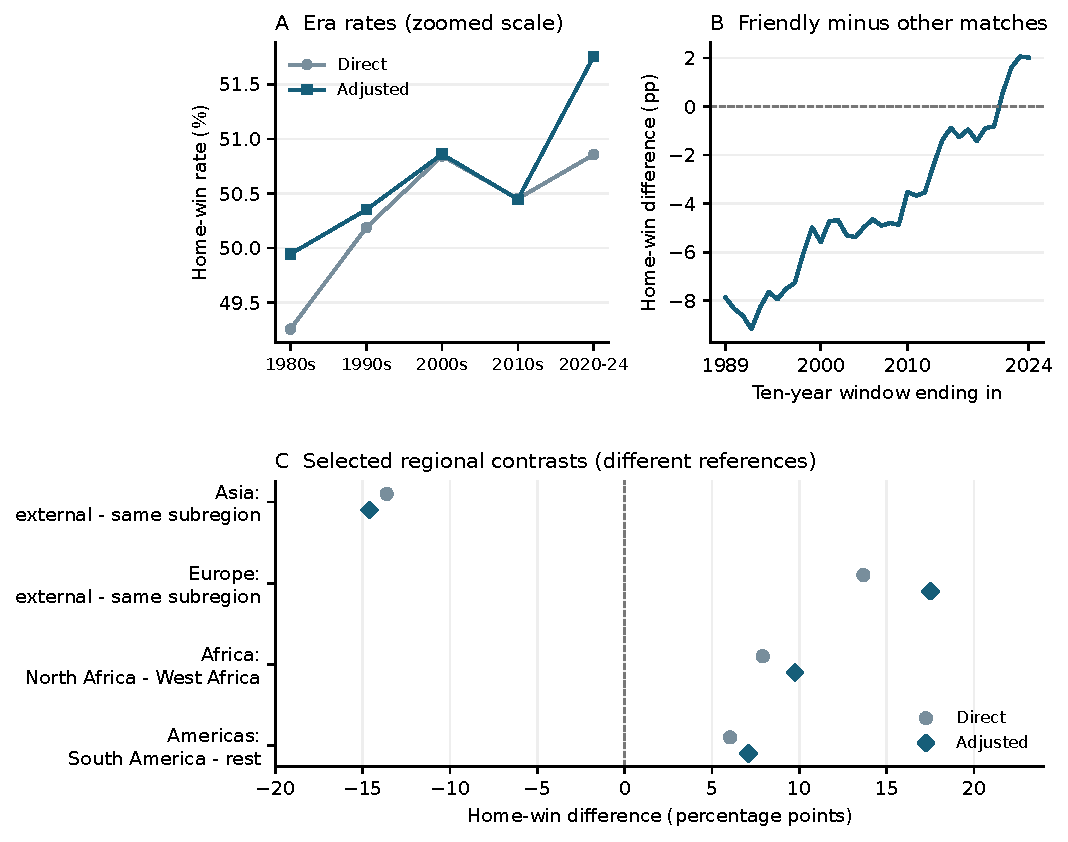
\includegraphics[width=\linewidth]{fig_historical_overview.pdf}
\papercaption{Historical patterns in the common 24,917-match cohort.}{(A) Direct and common-tournament-composition era rates; the vertical axis is truncated and the final era spans five years. (B) Direct friendly-minus-other gaps in 36 overlapping ten-year windows, indexed by ending year. (C) Four predefined regional contrasts: external opponents are outside the home continent; rest denotes other American subregions. Raw and adjusted contrasts use their specified references and do not constitute a regional ranking. The panels present descriptive estimates; uncertainty ranges are reported separately. Complete windows, 29 contrasts, and 155 directional matchups are indexed in the supporting-results guide.}
\label{fig:historical-overview}
\end{figure}

\begin{table}[htbp]
\centering\small
\papercaption{Selected contrasts in the 24,917-match historical sample, in percentage points.}{Ranges are model-conditional envelopes, not unconditional confidence intervals. Each adjustment uses its specified reference; the rows estimate different contrasts.}
\label{tab:historical-contrasts}
\begin{tabular}{p{7.4cm}rr}
\toprule
Contrast and adjustment & Estimate & Conditional range \\
\midrule
2010s minus 1980s, tournament composition & $+0.5019$ & $[-61.66,62.66]$ \\
2020--2024 minus 1980s, tournament composition & $+1.8100$ & $[-100,100]$ \\
Friendly minus other, direct & $-3.2463$ & --- \\
Friendly minus other, era composition & $-2.8831$ & $[-7.2039,1.4377]$ \\
\bottomrule
\end{tabular}
\end{table}

Regional differences depended on opponent composition. Asian home teams won $13.6160$~pp less often against opponents from outside Asia than against opponents from the same study subregion. These groups contained 1,743 and 1,934 matches; the adjusted difference was $-14.6057$~pp. This directional comparison uses the classifications in Section~\ref{sec:data-design}; it does not rank regional ability.

Of 29 predefined regional contrasts, 24 supported adjustment and five lacked required cells. Six of the 24 conditional ranges lay on one side of zero and 18 crossed it; missing comparisons were retained as unsupported. These contrasts are conditional on the observed schedules and reference distributions. Their interpretation also requires consideration of team strength.

The full regional output also contains 155 directional matchups: 153 have observations and 71 support the complete adjustment. Across the historical analyses, 198 of 292 registered targets received model-conditional ranges, while 94 lacked required cells. The 324 sensitivity scenarios produced 26,704 comparison rows; results for modified targets remain descriptive unless the calibration is repeated for those targets. Complete records are listed in the supporting-results guide.

% !TeX root = ../main.tex
\subsection{Strength Estimation: Development, Estimates, and Evaluation}
\label{sec:strength-development}

The strength model produces a time-indexed distribution of latent ability for each team. Figure~\ref{fig:strength-states} illustrates the output for four teams selected for presentation rather than predictive performance. Each point is a pre-match estimate that excludes the selected match's result and incorporates earlier home and away appearances. The means summarize estimated strength, while the whiskers show marginal uncertainty on the fixed performance-noise scale. These marginal summaries distinguish estimated ability from its uncertainty. The joint model uses the strength-difference mixture in Equation~\ref{eq:difference-mixture}, rather than only the displayed mean and standard deviation.

\begin{figure}[htbp]
\centering
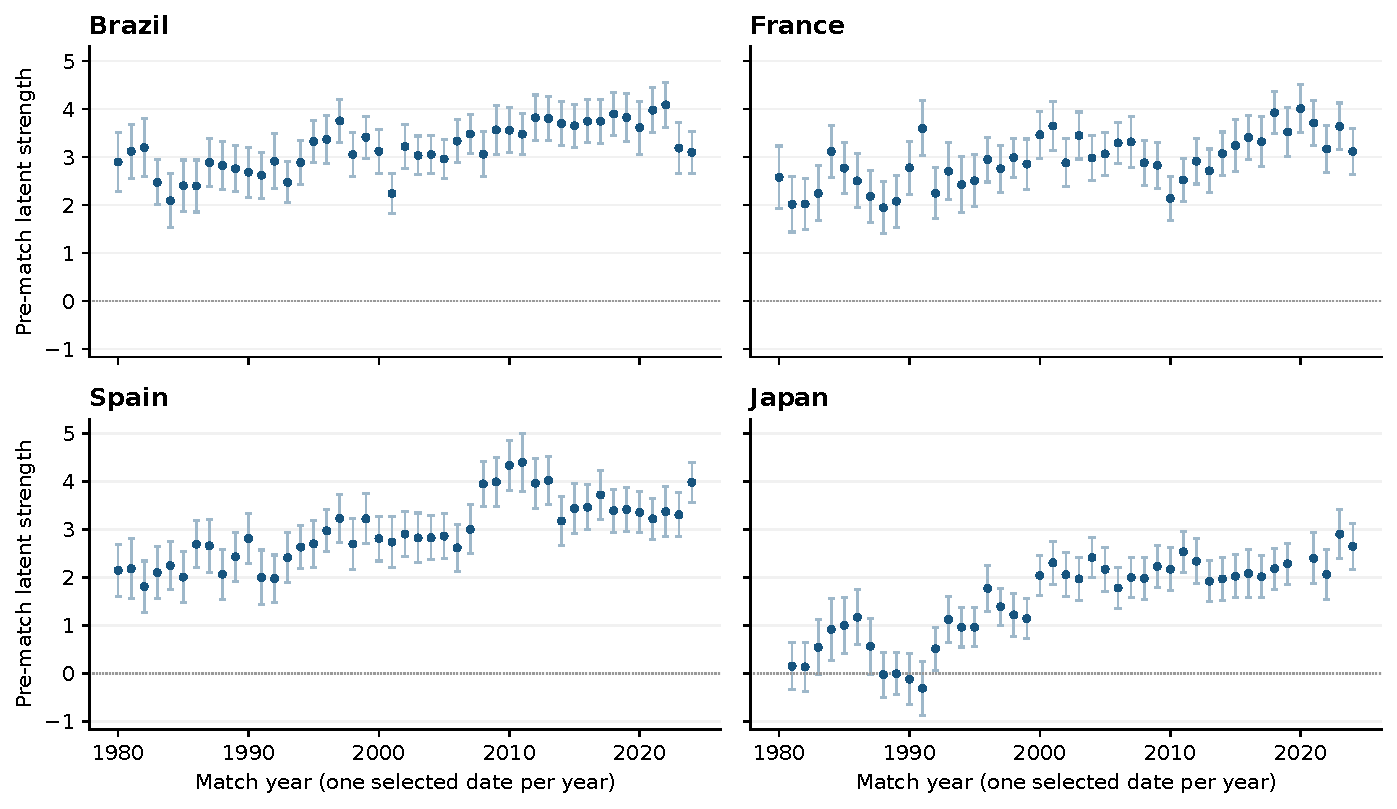
\includegraphics[width=\linewidth]{fig_strength_states.pdf}
\papercaption{Illustrative pre-match strength states, 1980--2024.}{For Brazil, France, Spain, and Japan, each point corresponds to the latest eligible comparative-cohort match in a year, considering both home and away appearances. Whiskers show the marginal mean plus or minus one standard deviation, including jump variance; they do not represent normal-quantile intervals or a world ranking. The zero line is the prior reference. Selected dates do not display every update, and gaps contain no interpolated state estimates.}
\label{fig:strength-states}
\end{figure}

\subsubsection{Model Revisions Informed by Development Results}

Development results informed revisions to the implementation and probability model. They do not establish the optimality of the final rating algorithm. First, explicit expansion of global jump combinations caused excessive memory use. A later moment-collapse approximation still differed from independent numerical references by about $1.328$~pp in match probability, above the original $1$~pp accuracy tolerance. The adopted implementation instead integrates local Poisson counts before processing results, shares a jump variable across a team's same-day matches, and retains the joint covariance. The maximum full-pipeline probability difference between the final ordinary and strict numerical settings was approximately $4.777\times10^{-7}$. This comparison assesses numerical stability for the recorded calculation, rather than the empirical validity of the latent process.

Second, improvements in overall probability scores did not eliminate bias in a particular friendly-match period. Earlier correction candidates underpredicted home wins in the 415 friendlies of 2020--2022 by approximately $3.32$--$4.51$~pp. Separate context fits, switching mixtures, and more flexible matrix corrections did not consistently satisfy the unchanged criteria. Diagnostics indicated distinct errors in probability shape and recent systematic offsets. The final pipeline therefore applies past-only shape correction followed by online residual correction, as described in Section~\ref{sec:strength-method}. For those 415 matches, underprediction decreased to $2.3913$~pp; the corresponding non-friendly bias was $-0.7689$~pp. For 2023--2024, friendly and other-match biases were $+0.9619$ and $+0.3622$~pp. These residual diagnostics do not estimate causal effects of tournament type.

The final comparison included eight candidates, combining two shape mappings with four residual-diffusion values. Two satisfied all prespecified criteria. With diffusion $0.02$, the shared-temperature version had a comparative-cohort loss of $0.890949$, compared with $0.891258$ for the matrix version. These aggregates cover the same 24,917 study matches, not the larger learning population. Candidates were first screened against the criteria, then compared by loss and structural simplicity. The shared-temperature version was selected. The historical data had already been used during development, so these scores do not constitute evaluation on an untouched final holdout. Failed candidates remain documented. The corrections improve the auxiliary probability branch; they do not retrospectively change the strength distributions delivered to the joint analysis.

\subsubsection{Three-Class Evaluation and Remaining Limitations}

Table~\ref{tab:rating-validation} reports the adopted rating-and-correction pipeline on four disjoint historical periods of the comparative cohort. Its target is home win, draw, or away win. The frequency baseline uses earlier venue-specific outcome counts; the internal fixed-step baseline updates both teams from expected-score errors and uses a Davidson-form draw probability. Its registered settings are update size $40$, home offset $100$, and draw parameter $0.75$, on its own rating scale. This internal comparator uses Elo-style updates and is distinct from the official FIFA system. All three issue probabilities before learning the current date's results.

\begin{table}[htbp]
\centering\small
\papercaption{Three-class performance of the final rating pipeline on the comparative cohort.}{The four periods partition 24,917 matches. Loss is three-class negative log probability of the actual result; accuracy selects the most probable of the three outcomes. Bias is predicted minus observed home-win frequency in pp. These results include the probability corrections and reuse development history. They are not directly comparable with the binary scores in Table~\ref{tab:predictive-models}.}
\label{tab:rating-validation}
\begin{tabular*}{\linewidth}{@{\extracolsep{\fill}}lrrrrrr@{}}
\toprule
Period & $n$ & Frequency & Fixed-step & Adopted & Accuracy (\%) & Bias (pp) \\
\midrule
1980--1999 & 8,318 & 1.042385 & 0.939775 & 0.917339 & 56.30 & $+0.1807$ \\
2000--2009 & 6,872 & 1.033723 & 0.895936 & 0.880976 & 59.02 & $-0.0173$ \\
2010--2019 & 6,632 & 1.035877 & 0.880793 & 0.878495 & 60.00 & $+0.0047$ \\
2020--2024 & 3,095 & 1.032750 & 0.863959 & 0.868851 & 60.26 & $-0.3910$ \\
\bottomrule
\end{tabular*}

\end{table}

The pipeline had lower loss than the frequency comparator in every displayed period and lower loss than the fixed-step comparator in the first three. However, in 2020--2024 its loss is $0.868851$ versus $0.863959$, and its accuracy is $60.26\%$ versus $60.97\%$. The loss difference satisfies the prespecified $0.01$ non-inferiority tolerance, although the selected pipeline did not outperform the baseline in every period. The requirements also checked loss improvement of at least $0.005$ against frequency, accuracy no more than $1$~pp below frequency, absolute home-win bias at most $3$~pp, and probability-bin error at most $10$~pp for bins with at least 200 games. Satisfying these tolerances establishes compliance with the operational criteria, rather than general superiority or calibration in every subgroup.

The validation records include 63 targeted tests, independent integration checks, full-history replay, and checkpoint continuation. Simulation under two alternative jump-parameter settings gave nominal $90\%$ strength-difference range coverage of approximately $95.90\%$ and $92.65\%$. These checks assess implementation consistency, numerical approximation, and performance under specified simulation settings. They do not provide observed true-strength labels for real teams. Initialization checks also found 2,905 study matches with a raw home-probability change exceeding $1$~pp under at least one registered alternative, 359 cold starts, and 80 matches whose prior cumulative opponent graph was disconnected. Some match-level initialization effects were substantially larger than the average. The corresponding flags and uncertainty information are retained because a common rating scale does not imply equally reliable comparisons across teams and regions.

The latent strength distributions provide the input to the joint analysis, with the limitations identified above. Corrected three-class probabilities serve as a separate forecasting diagnostic. The common-sample comparison below evaluates the contribution of strength to the binary home-win target and the additional contribution of context.


\subsection{Strength versus Context}
\label{sec:strength-results}
% E32_M0_nested/M1_strength/M3_nested, E32_CONTEXT_*, E32_ADMISSION.

For RQ2, we evaluated background-only, strength-only, and joint predictors on the same 21,413 matches from 1990--2024, using only information available before each prediction. This is a retrospective chronological comparison: the archive also informed development and selection, as described in Section~\ref{sec:data-design}.

Including strength produced the larger reduction in loss (Table~\ref{tab:predictive-models}; Figure~\ref{fig:predictive-models}). Mean log loss declined from $0.671936$ for background alone to $0.566020$ for strength alone and $0.563630$ for the joint predictor. The joint model's relative reductions were $16.12\%$ against background alone and $0.42\%$ against strength alone. The absolute reductions were 0.105916 from background to strength and 0.002390 from strength to the joint model. These are aggregate loss comparisons, not an additive decomposition of information or evidence for individual subgroups. Binary accuracy followed the same ordering: $58.19\%$, $69.83\%$, and $70.01\%$. Accuracy refers to home-win/non-home-win classification and is distinct from relative loss reduction.

\begin{table}[htbp]
\centering\small
\papercaption{Same-match retrospective comparison, 1990--2024 ($n=21,413$).}{Bias is mean predicted home-win probability minus the observed rate, in percentage points. Lower loss and Brier score are preferable.}
\label{tab:predictive-models}
\begin{tabular}{lrrrr}
\toprule
Predictor & Log loss & Brier score & Accuracy (\%) & Bias (pp) \\
\midrule
Background only & 0.671936 & 0.239580 & 58.19 & $-0.0973$ \\
Strength only & 0.566020 & 0.193698 & 69.83 & $+0.9308$ \\
Strength and context & 0.563630 & 0.192657 & 70.01 & $+0.2398$ \\
\bottomrule
\end{tabular}
\end{table}

Adding context also reduced the Brier score from $0.193698$ to $0.192657$ and mean bias from $+0.9308$ to $+0.2398$~pp. The background-only model had the smallest absolute mean bias but the highest loss and Brier score. Agreement with the overall frequency therefore does not establish match-level predictive quality or calibration across probability levels and groups.

\begin{figure}[htbp]
\centering
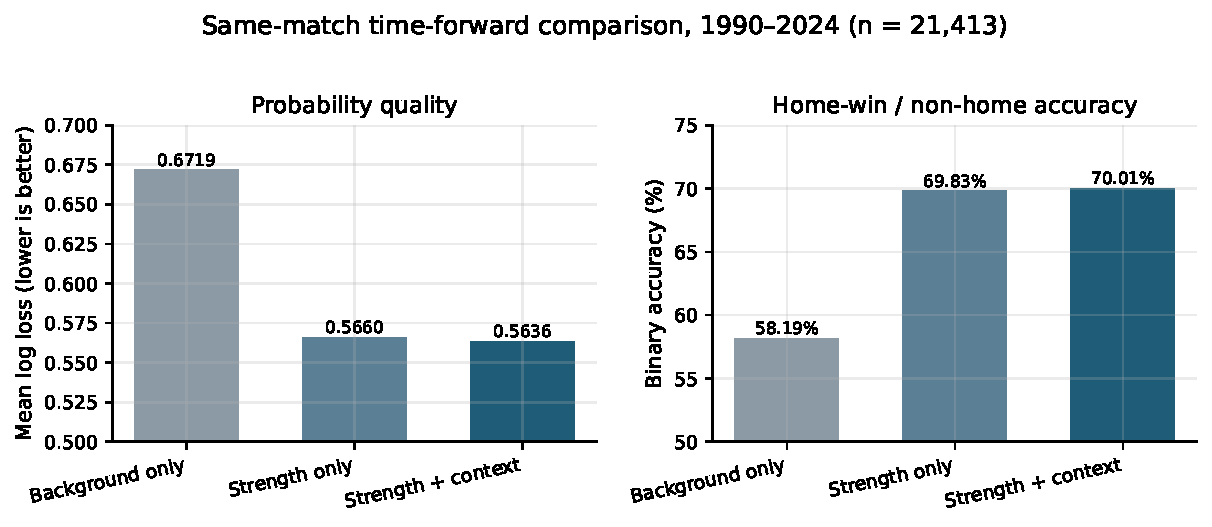
\includegraphics[width=\linewidth]{fig3_model_comparison.pdf}
\papercaption{Strength accounts for most of the improvement in the same-match historical comparison ($n=21,413$, 1990--2024).}{Adding context yields a smaller reduction in loss. Both vertical axes are truncated; magnitudes should be read from the labelled values rather than bar-height ratios. Accuracy is binary; no dependence-adjusted interval from real match data is available for the loss difference.}
\label{fig:predictive-models}
\end{figure}

The separate conditional analysis uses 24,917 matches and a fixed reference. Its strength-adjusted friendly-minus-other contrast was $-3.4957$~pp, with a range from $-7.6712$ to $0.6797$~pp. The paired change after adding strength was $+0.3624$~pp, ranging from $-2.8619$ to $3.5868$~pp. The estimated change was small, and its conditional range did not resolve its direction. Because the reference and target differ, these values cannot be subtracted from the descriptive contrast in Table~\ref{tab:historical-contrasts}.

Of 54 principal quantities assessed by simulation, 30 met the acceptance criteria. For 24 regional changes before and after strength adjustment, the simulated reference values were insufficiently precise for interval validation. These changes remain descriptive; failure to meet the validation criterion does not imply an absence of regional differences. The selected complete-history procedure evaluates conditional comparisons under the specified generators (Section~\ref{sec:evaluation-method}). The separate $0.42\%$ predictive loss gain has no dependence-adjusted interval from real match data, so its persistence in future matches is unresolved.

\subsection{Historical Information and Computational Trade-offs}
\label{sec:history-results}
% E33_LOSS_*, E33_COST_*, E33_SIX_COMBINATIONS, E33_ADAPTIVE.

For RQ3, the historical window used for strength reconstruction was varied separately from the window used to estimate outcome probabilities. Evaluation covered 16,599 matches in 2000--2024, with 9,727 in the main 2010--2024 comparison. Among six tested combinations, cumulative history at both stages gave the lowest main-comparison log loss, $0.559135$ (Figure~\ref{fig:history-windows}). Annual selection using past performance gave $0.560159$. Cumulative history was therefore retained among the tested choices. Earlier matches need not have equal influence on current estimates because the dynamic strength process allows ability to change.

A 12-year outcome-learning window, with cumulative strength estimation fixed, increased loss from $0.559135$ to $0.561131$, or $0.3571\%$ using unrounded values. In the controlled timing batch, this component took $105.29$ rather than $312.58$ seconds, a $66.31\%$ saving. The saving applies to this outcome-fitting component. Other timings in Figure~\ref{fig:history-windows} were obtained in different execution batches and are not standardized benchmarks of the complete pipeline.

\begin{figure}[htbp]
\centering
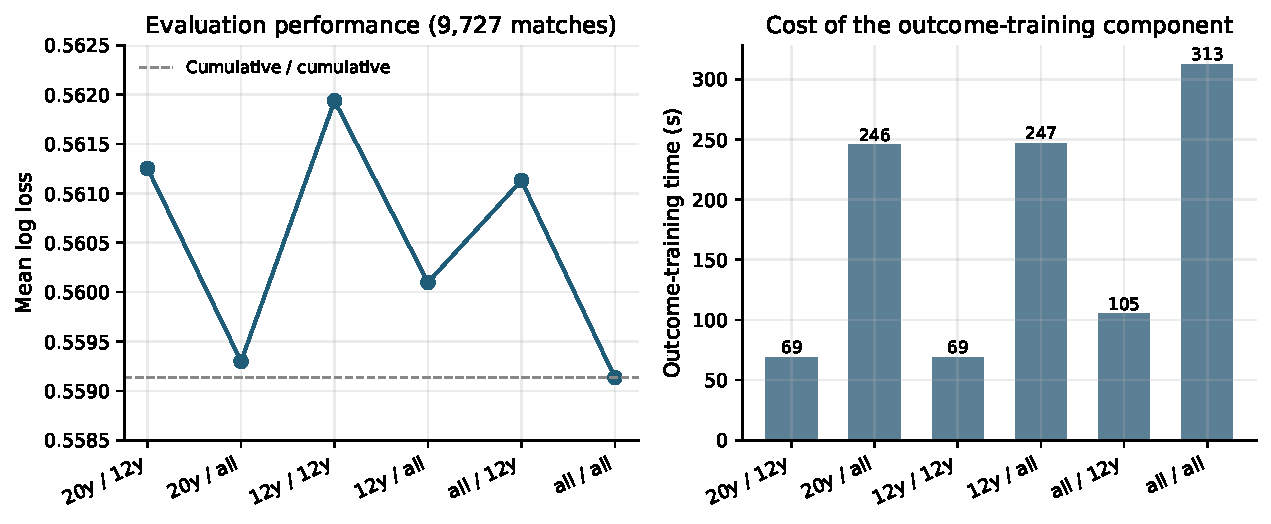
\includegraphics[width=\linewidth]{fig4_history_windows.pdf}
\papercaption{Six tested combinations of rating memory and outcome-learning history.}{Left: loss on the common 2010--2024 sample ($n=9,727$); lines connect discrete candidates for visual reference only. Right: recorded outcome-learning component times, not total pipeline times. The controlled saving in the text compares only all/12y with all/all; timings from other execution batches are not standardized.}
\label{fig:history-windows}
\end{figure}

\subsection{Regional Applicability and Probability Bias}
\label{sec:regional-results}
% E34_*; calibration and composition evidence extended in R20261106-05.

Regional applicability of the joint predictor was assessed using the same 9,727-match main sample. Overall, its log loss was $0.559135$, compared with $0.562000$ for strength alone. This later-period comparison is separate from the 21,413-match evaluation above. Regional scores and bias varied (Table~\ref{tab:regional-diagnostics}; Figure~\ref{fig:regional-metrics}), alongside differences in opponent composition and strength uncertainty. These scores describe performance on the observed matches and do not measure the intrinsic difficulty or quality of a region.

\begin{table}[htbp]
\centering\small
\papercaption{Regional diagnostics, 2010--2024.}{Losses compare identical matches within each row; bias concerns the joint predictor, in percentage points. Interpretations summarize the specified sensitivity checks and do not constitute confidence statements or regional rankings. Americas includes South America; Overall is not an independent additional sample.}
\label{tab:regional-diagnostics}
\begin{tabular}{lrrrrp{3.4cm}}
\toprule
Home region & $n$ & Strength loss & Joint loss & Bias (pp) & Interpretation \\
\midrule
Europe & 3,322 & 0.543239 & 0.539498 & $+0.2189$ & Increment retained \\
Asia & 2,540 & 0.546894 & 0.545041 & $-0.8765$ & Increment retained \\
Africa & 2,058 & 0.613617 & 0.612607 & $+0.6854$ & Increment sensitive \\
Americas & 1,659 & 0.559276 & 0.554578 & $+0.1858$ & Increment retained \\
Oceania & 148 & 0.555130 & 0.549289 & $+2.9572$ & Sparse support \\
Overall & 9,727 & 0.562000 & 0.559135 & $+0.0676$ & Pooled comparison \\
\bottomrule
\end{tabular}
\end{table}

The small loss reductions from adding context in Europe, Asia, and the Americas retained their direction under the specified year/team deletions and alternative reference distributions. These checks provide limited historical support for the additional predictive value of context in these regions. The African increment was more sensitive: its sign reversed after removing 2011 or evaluation matches involving Egypt. This sensitivity concerns the incremental value of context, rather than the predictive value of strength itself in Africa.

The African results also show that a small overall bias can coexist with errors within probability groups. In the low strength-uncertainty category, the 20--40\% predicted-probability bin contained 225 matches, with mean predicted probability $31.21\%$ and observed home-win rate $34.22\%$. In the 60--80\% bin, 287 matches had mean predicted probability $69.17\%$ and observed rate $65.85\%$. The lower bin was underpredicted and the higher bin overpredicted; these directions persisted in the specified checks. Standardizing the broad strength-gap and uncertainty composition narrowed the Africa--Europe loss gap but did not remove it. The remaining discrepancy warrants further investigation, but these comparisons do not identify its cause or demonstrate that uncertainty is fully represented.

South America's ordering relative to the rest of the Americas changed under some deletions and alternative reference distributions. In Oceania, 148 matches were spread over nine adjustment cells, one containing only two matches; deleting matches involving certain teams left a required cell empty. The adjusted comparison was consequently sensitive to a few observations and could become unsupported. These checks held predictions fixed: they did not erase deleted matches from the original learning history or refit each model. They assess the sensitivity of evaluation summaries with predictions held fixed, rather than the performance of a retrained system, and do not yield real-world confidence intervals.

\begin{figure}[htbp]
\centering
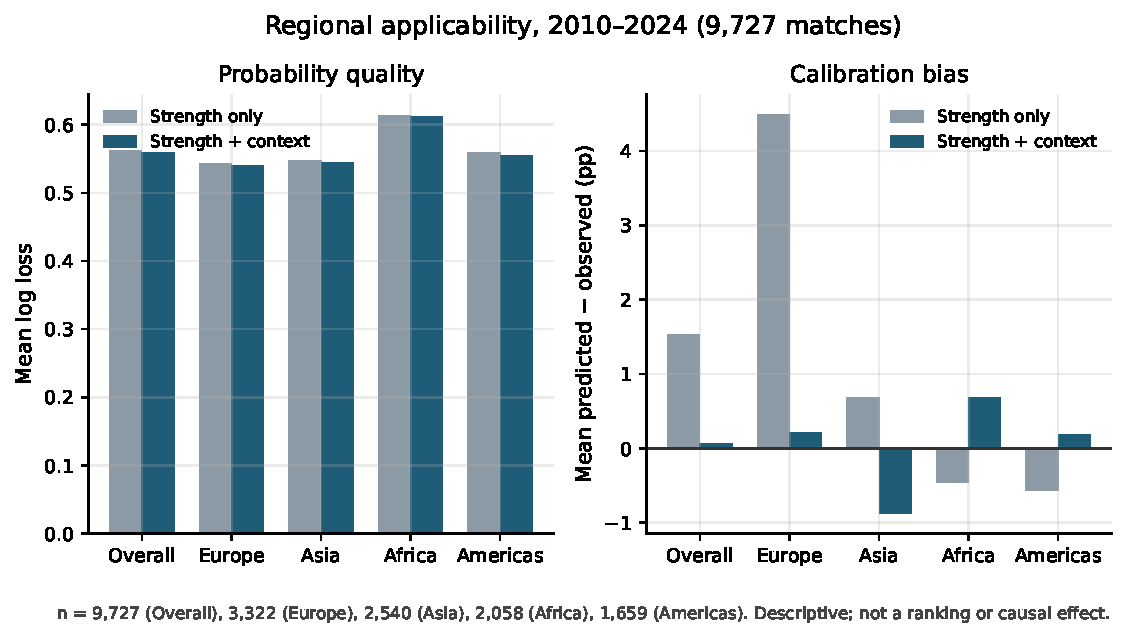
\includegraphics[width=\linewidth]{fig5_regional_metrics.pdf}
\papercaption{Regional probability quality and mean bias on the main 2010--2024 sample.}{The displayed regional groups contain 9,579 of 9,727 matches; Overall additionally includes Oceania's 148 matches. Positive bias means average overprediction. The sensitivity checks discussed in the text supplement these point scores; the scores alone do not establish stable improvements.}
\label{fig:regional-metrics}
\end{figure}

\subsection{Prospective Application}
\label{sec:prospective-results}
% E35_ISSUED and E35_CASE_005/010/048/CZE_SPA.

We applied the model to 52 Nations League fixtures scheduled for 12--17 November 2026 and archived the release on 2 November at 04:07:15 UTC. Dates and pairings were taken from UEFA's schedule~\cite{uefa2026fixtures} and frozen in the issued fixture ledger. Strength estimates used accepted results through 6 October 2026; outcome-model coefficient estimation used data through 29 December 2025. Predictions for both rounds use the same information set. The joint model issued 49 binary predictions and withheld three involving third-country venues outside its application rule. The rating model separately supplied auxiliary win--draw--loss probabilities for all 52 targets; these auxiliary outputs do not replace the withheld joint predictions. The auxiliary three-class outputs are outside the binary model comparison and have not received prospective validation in this release.

Of the 49 joint predictions, 21 favoured a home win and 28 a non-home win; 32 strength-induced ranges crossed the $50\%$ decision threshold. England--Croatia had home-win probability $63.50\%$ (range $43.54$--$81.28\%$); Netherlands--Greece had $50.38\%$ ($31.02$--$69.68\%$); and Czech Republic--Spain had $3.83\%$ ($0.76$--$9.38\%$). For Ukraine--Georgia, the joint estimate was withheld and auxiliary home/draw/away probabilities were $52.26\%$, $25.39\%$, and $22.35\%$. Figure~\ref{fig:issued-forecasts} displays central 90\% ranges from latent strength uncertainty with coefficients fixed; they exclude parameter and model error.

\begin{figure}[htbp]
\centering
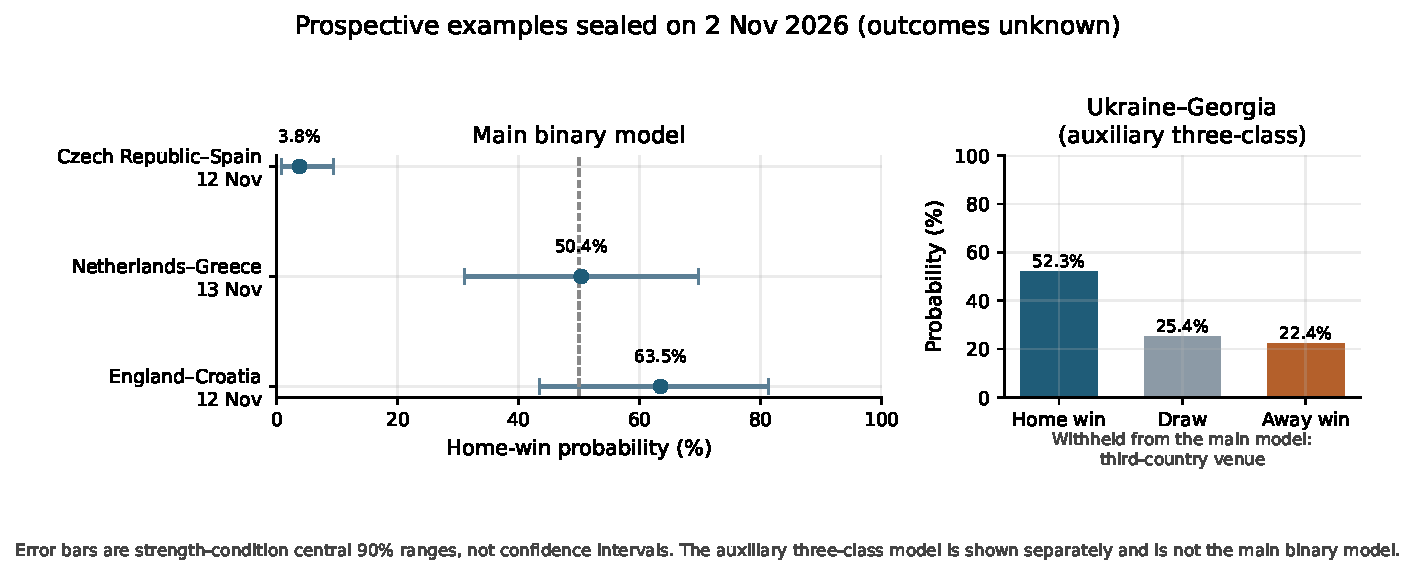
\includegraphics[width=\linewidth]{fig6_forecast_examples.pdf}
\papercaption{Examples from the sealed 2 November 2026 release for 12--17 November fixtures.}{Left: joint binary probabilities with fixed-coefficient latent-strength central 90\% ranges. Right: auxiliary native win--draw--loss probabilities for Ukraine--Georgia, for which the main model withheld its estimate under the venue rule. Actual outcomes are absent; Table~\ref{tab:predictive-models}'s historical accuracy is not an accuracy estimate for these fixtures.}
\label{fig:issued-forecasts}
\end{figure}

The release documents prospective application, with outcomes excluded from the archived ledger. Predictive performance on these fixtures remains unevaluated.

% Final placement is checked in the rendered PDF; no forced float-only page.

% !TeX root = ../main.tex
% Language revision R20261107-10; numerical and inferential scope retained.
\section{Discussion and Conclusion}
\subsection{Findings and Contributions}

For RQ1, adjustment for era composition reduced the friendly--other-match gap, and geographic comparisons depended on the opponents represented. Several model-conditional ranges were too broad to resolve the direction of a difference. These comparisons provide a common descriptive basis for the strength-adjusted analysis, without identifying a pure home effect or a universal regional ranking.

For RQ2, the larger reduction in aggregate loss was associated with strength, while context provided a smaller increment. Dynamic paired comparisons~\citep{glickman1999dynamic} convert earlier results into estimates of ability and uncertainty; the common-sample comparison then tests whether context improves predictions beyond those estimates. The result gives context a conditional forecasting role. It does not turn geographic or tournament differences in observed home-win rates into an independent measure of venue advantage.

For RQ3, cumulative history performed best in the main comparison among the tested choices and remains the default. A shorter outcome-fitting window reduced computation at a small predictive cost. Regional diagnostics qualified the aggregate context gain: in Africa, its direction was sensitive to particular years and teams, while opposing probability biases persisted in selected uncertainty groups. These findings identify specific targets for further evaluation and calibration.

The project's contribution is the integration of match and identity curation, a date-ordered strength-estimation and prediction implementation, and common-sample evaluation of contextual information. The paired-comparison, approximate-inference, calibration, and scoring principles are drawn from the cited literature; methodological integration and empirical analysis, rather than the invention of those principles, distinguish this work. Documented information dates and an explicit withholding rule connect the historical analysis to prospective application. Proper probability scores~\citep{gneiting2007scoring} identify differences that mean bias or accuracy alone may obscure. The archived release permits subsequent evaluation against outcomes unavailable at issue time.

\subsection{Limitations}

The findings apply to the documented study population. Some historical identity and membership decisions rely on records accepted by the project lead, and the full archive has not been independently verified. Geographic classifications include study-specific overrides, while sparse opponent combinations limit comparability. Because some scores include extra time, the target cannot consistently be interpreted as a regulation-time result.

Approximate strength inference, assumed jump dynamics, and restricted context terms may leave substantial variation unexplained. The conditional comparisons do not account for all differences in travel, team selection, venues, or match importance. The main model combines draws and away wins, whereas the auxiliary model distinguishes three outcomes; their classification accuracies address different targets.

Some limitations have measurable consequences. The ordinary and strict numerical replays differed little, whereas initialization alternatives changed raw probabilities by more than $1$~pp in 2,905 study matches. These changes measure sensitivity and do not provide additional confidence bounds for corrected predictions. The final pipeline's recent-period loss was also slightly higher than that of the fixed-step baseline, limiting claims about the benefit of persistent jumps and probability correction. The separate effects of Gaussian projection, unmeasured squad changes, weak cross-region connections, and historical identity errors have not been quantified.

Development results changed both the integration procedure and probability correction: numerical-reference failures prompted a new integration order, and residual bias prompted separate shape and drift corrections. These revisions addressed observed defects under the documented criteria. Because the same archive also informed those decisions, the resulting historical scores can favor revisions specific to that archive. The prospective release preserves predictions made before their outcomes and permits a later test on new matches.

Chronological prediction excludes each match's own outcome from its inputs, but it does not make a reused development archive an untouched final test. Simulation results apply to their specified generators, and no dependence-adjusted interval from real match data establishes the persistence of the small contextual gain. Deletion checks assess evaluation composition while retaining the original learning history. Prospective evaluation and regional diagnostics therefore address different remaining questions about model use.

The historical uncertainty procedure also failed under a permanent global-shock generator. Its envelopes therefore remain conditional on the generating mechanisms for which the procedure met the validation criteria, rather than providing guarantees for arbitrary football histories.

\subsection{Future Work}

Four extensions warrant investigation. First, a three-class joint model could use a draw interval, as in TrueSkill~\citep{herbrich2006trueskill}, or divide non-home-win probability between draws and away wins. Both formulations require evaluation against the existing auxiliary model.

Second, calibration mappings learned from earlier predictions and outcomes could reduce systematic bias. Temperature scaling~\citep{guo2017calibration} is one candidate, although its published evidence concerns neural classifiers. Benefits require chronological and regional evaluation, and improved calibration need not improve classification accuracy.

Third, goal-based models~\citep{dixon1997scores} could estimate richer outcomes, subject to consistent score definitions and joint treatment of scores and match results. Verified venue or squad information must be available before prediction. These variables remain untested explanations of the observed biases.

Fourth, club-football analysis requires new ratings and parameters for seasons, transfers, promotion and relegation, and connections between leagues. An initial single-league study could model seasonal transitions explicitly. The predictive benefits of these proposed extensions remain unestablished.

\subsection{Conclusion}

Within this international-football archive, strength provided the larger reduction in predictive loss, and context supplied a smaller increment whose stability varied across regional checks. Historical-window comparisons favored cumulative history among the tested choices and identified a computation--prediction trade-off. These results support evaluating historical home-win patterns as additional forecasting information after accounting for uncertain strength. The archived prospective release applies that approach with explicit information dates and preserves its probabilities for evaluation when outcomes become available.

\section*{Declarations}
\phantomsection\addcontentsline{toc}{section}{Declarations}
\paragraph{Data and code availability.}
Source match data are available under CC0 from martj42~\citep{martj42_data}. The accompanying repository provides code, configurations, build instructions, experiment records, and input/output fingerprints identifying the reported versions.

The English guide \path{paper/SUPPORTING_RESULTS.md} indexes all stage tables, methods, reproduction instructions, windows, geographic matchups, sensitivity outputs, and the 52-fixture forecast ledger. The main text reports selected results.

\paragraph{Team responsibilities.}
The division of responsibilities was as follows: Ruiyi Gao was responsible for study design, coordination, computational analysis, and manuscript preparation; Zhenglin Chen for code review and methodological refinement; and Wenyu Jiang for supplementary data collection and presentation preparation.

\paragraph{Use of AI-assisted tools.}
AI-assisted tools supported code development, documentation, and manuscript revision. Empirical claims are supported by the archived data and computational outputs, rather than by generated text alone.

\begingroup
\fontsize{10}{11}\selectfont
\setlength{\emergencystretch}{2em}
\setlength{\bibsep}{1pt}
\interlinepenalty=10000
\bibliographystyle{unsrtnat}
\bibliography{references}
\endgroup
\end{document}
